\begin{center}
	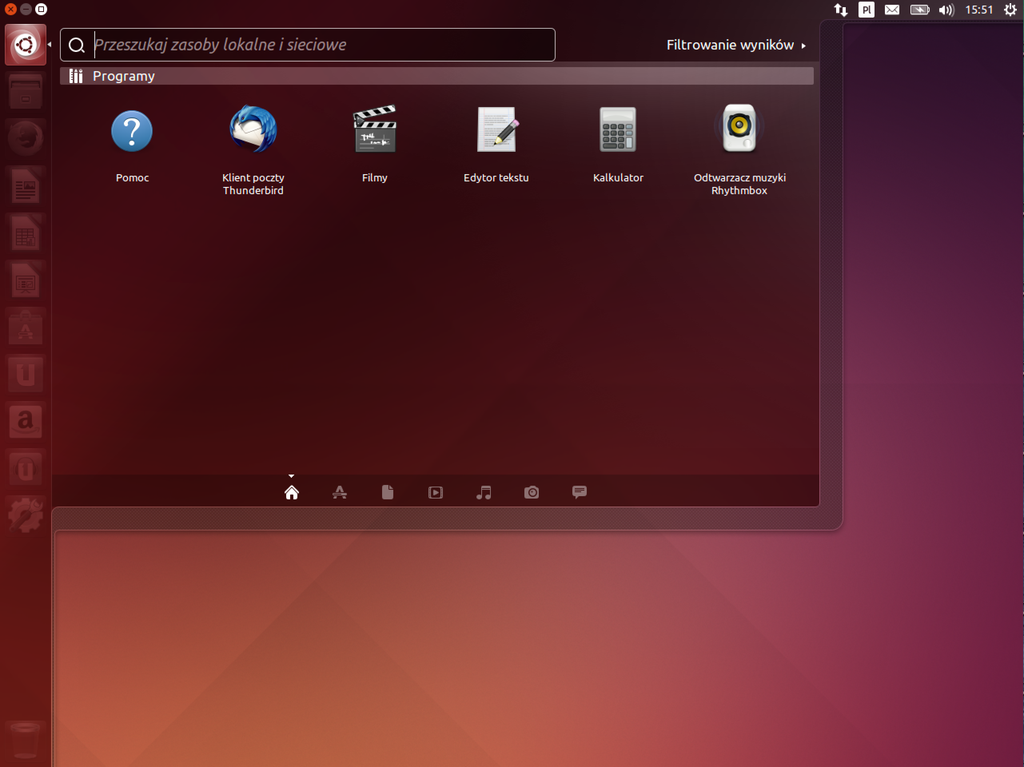
\includegraphics[width=\linewidth]{images/unity_pulpit_dash.png}
\end{center}

Dash jest potężnym narzędziem w Unity, które w szybki sposób pozwala nam na dostęp i wyszukiwanie programów, plików oraz dodatkowych informacji przechowywanych nie tylko w naszym komputerze (zainstalowane programy, ostatnio używane dokumenty, zakładki i ostatnio odwiedzone strony i inne), ale również informacji dostępnych w sieci (Twitter, Facebook, Google Docs, Youtube, Wikipedia, Amazon i inne). Wyniki wyszukiwania w zewnętrznych serwisach dopasowane są do wyszukiwanej frazy i zwracane są w oknie Dasha. Jeżeli przejmujesz się tym, że szukana fraza przesyłana do Internetu, to funkcjonalność ta może zostać wyłączona w Ustawieniach systemowych w oknie \textcolor{ubuntu_orange}{Prywatność i bezpieczeństwo.}

Dash można porównać do Menu Start z systemu Microsoft Windows XP/Vista/7 lub do ekranu startowego w Windows 8. Odpowiednikiem Dasha w systemie OS X jest Launchpad.

\begin{wrapfigure}{l}{0.1\textwidth}
                
\includegraphics[width=\linewidth]{images/ikony_dash.png}
\end{wrapfigure}

Ikona Dasha umieszczona jest na pierwszej pozycji na pasku Launchera – jest ona dość charakterystyczna i zawiera logo Ubuntu. Po naciśnięciu na ikonę Dasha naszym oczom ukaże się jego przezroczyste okno, które w swojej środkowej części okna wyświetla dwie grupy: ostatnio uruchomionych programów oraz ostatnio przeglądanych i pobranych plików oraz katalogów, a także wyszukiwanych informacji. W górnej części Dasha znajduje się pasek wyszukiwania, który nie tylko pozwala przeszukiwać zasoby komputera, ale pozwala również wyszukiwać i przeglądać informacje z popularnych serwisów w sieci. 

\begin{wrapfigure}{l}{0.2\textwidth}
                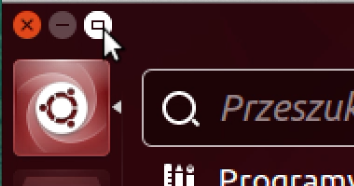
\includegraphics[width=\linewidth]{images/unity_dash_max.png}
\end{wrapfigure}

Dash po uruchomieniu zajmuje pewien obszar ekranu. Okno to można powiększyć do pełnego rozmiaru ekranu – służy do tego przycisk maksymalizacji w lewym górnym rogu, który jest widoczny, gdy Dash jest wywołany.\\
Wyszukiwanie w pasku jest dynamiczne i rezultaty zmieniają się podczas wpisywania tekstu. Wyniki w Dashu można filtrować. Służy do tego nie tylko przycisk Filtrowania wyników, ale również domyślnie włączone soczewki (Lenses).

\subsubsection{Soczewki (Lenses)}
\begin{center}
	
\includegraphics[width=\linewidth]{images/unity_dash_lenses.png}
\end{center}

Domyślnie w systemie dostępnych jest siedem soczewek i umieszczone są one na dole okna Dasha. Aktualnie wybrana soczewka jest jaśniejsza od pozostałych oraz ma nas sobą niewielki trójkącik. Soczewki służą do ograniczania wyników wyszukiwania do konkretnych kategorii.
\begin{description}
\item[
\includegraphics{images/unity_dash_lens_home.png}] \textcolor{ubuntu_orange}{Soczewka domowa} zawiera wszystkie wyniki wyszukiwania. 
\item[
\includegraphics{images/unity_dash_lens_programy.png}]\textcolor{ubuntu_orange}{Soczewka programów} zawiera wyniki wyszukiwania programów.
\item[
\includegraphics{images/unity_dash_lens_pliki.png}] \textcolor{ubuntu_orange}{Soczewka plików} zawiera wyniki wyszukiwania w plikach i katalogach.
\item[
\includegraphics{images/unity_dash_lens_video.png}] \textcolor{ubuntu_orange}{Soczewka filmów} zawiera wyniki wyszukiwania filmów.
\item[
\includegraphics{images/unity_dash_lens_audio.png}] \textcolor{ubuntu_orange}{Soczewka muzyki} zawiera wyniki wyszukiwania muzyki.
\item[
\includegraphics{images/unity_dash_lens_photo.png}] \textcolor{ubuntu_orange}{Soczewka zdjęć} zawiera wyniki wyszukiwania w fotografiach.
\item[
\includegraphics{images/unity_dash_lens_social.png}] \textbf{Soczewka społecznościowa} zawiera wyniki wyszukiwania w serwisach społecznościowych do których jesteś zalogowany.
\end{description}

Soczewka domowa ma wiele zastosowań i oprócz wcześniej wspomnianych możliwości, możemy ją wykorzystać do wyszukania informacji na przykład w Wikipedii, Google lub możemy wyszukać informacji na temat pogody w naszym regionie.
\clearpage
\begin{center}
	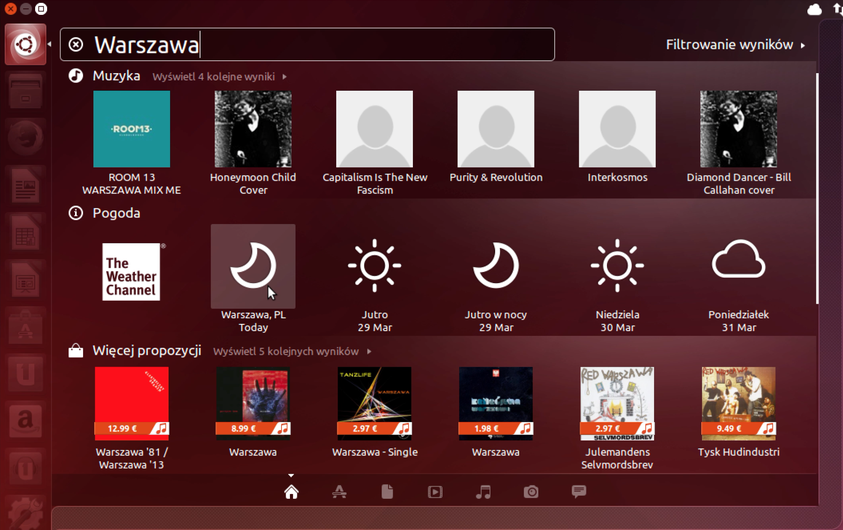
\includegraphics[width=\linewidth]{images/unity_dash_wyszukiwanie.png}
\end{center}

Aby uzyskać więcej informacji, nie trzeba od razu otwierać wyniku. Naciśnięcie prawym przyciskiem myszy którymś z wyników wyszukiwania, poda nam więcej informacji.

\begin{center}
	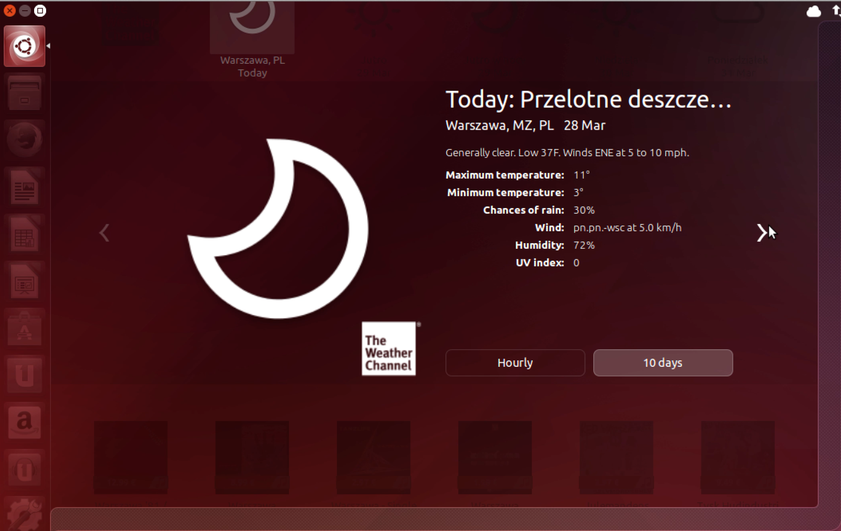
\includegraphics[width=\linewidth]{images/unity_dash_wyszukiwanie2.png}
\end{center}

Wyniki wyszukiwania można zawęzić do konkretnych źródeł wykorzystując do tego przycisk Filtrowania wyników. Podobnie jest w przypadku wyszukiwania informacji z wykorzystaniem pozostałych soczewek.

\begin{center}
	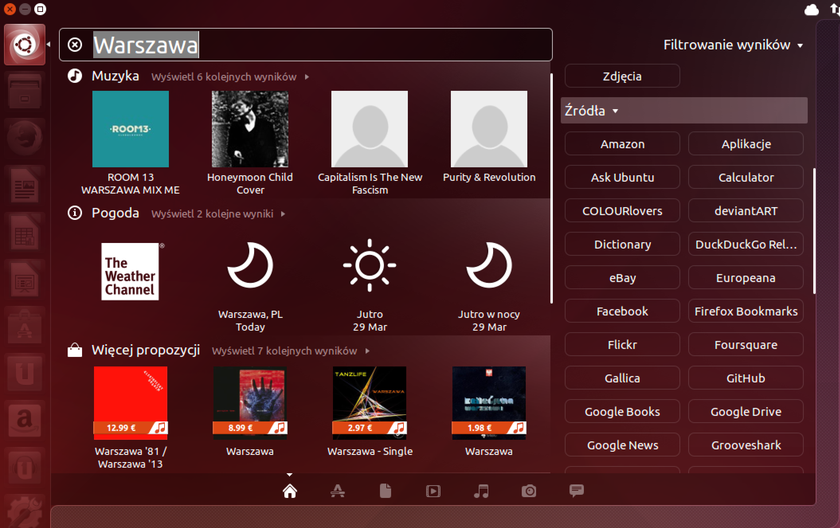
\includegraphics[width=\linewidth]{images/unity_dash_wyszukiwanie3.png}
\end{center}

W Ubuntu nie jesteśmy limitowani jedynie zainstalowanymi soczewkami. Wiele serwisów Internetowych udostępnia swoje własne soczewki, które można w łatwy sposób doinstalować i korzystać z nich w ten sam sposób, jak z domyślnie dostępnych.
%TODO opisać instalację soczewki.